\documentclass{standalone}

\usepackage[svgnames]{xcolor}
\usepackage{tikz}
\usepackage{pgfplots}
\usetikzlibrary{arrows.meta,plotmarks,calc,spath3}
\usepgfplotslibrary{fillbetween}
\pgfplotsset{compat = 1.18}

\begin{document}

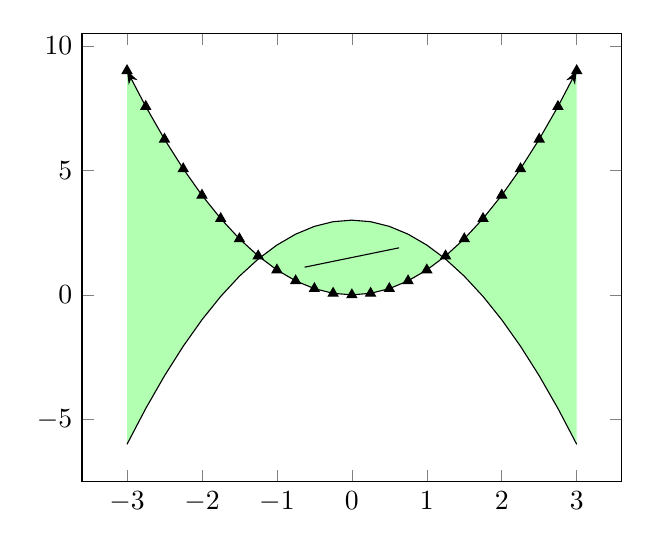
\begin{tikzpicture}
	\begin{axis}
		\addplot[name path=pathA, domain=-3:3, draw=none, mark=triangle*] {(x^2)};
		\draw[{Stealth}-{Stealth}, spath/use=pathA];
		\draw ($(-1, 0) + (10pt, 10pt)$) -- ($(1, 3) - (10pt, 10pt)$);
		\addplot[name path=pathB, domain=-3:3] {(-x^2 + 3)};
		\addplot[green, fill opacity=0.3] fill between[of=pathA and pathB];
	\end{axis}
\end{tikzpicture}

\end{document}
